% Full instructions available at:
% https://github.com/elauksap/focus-beamertheme

\documentclass{beamer}
\usetheme{focus}

\usepackage{wrapfig}
\usepackage{csquotes}
\usepackage{listings}
\usepackage{verbatim}
\usepackage{hyperref}

\AtBeginSection[]
{
  \begin{frame}
    \frametitle{Table of Contents}
    \tableofcontents[currentsection]
  \end{frame}
}

\title{Using LaTeX and Markdown for Reproducible Research}
\subtitle{}
\author{Erik Beck \\ Emily Y. Li}
\titlegraphic{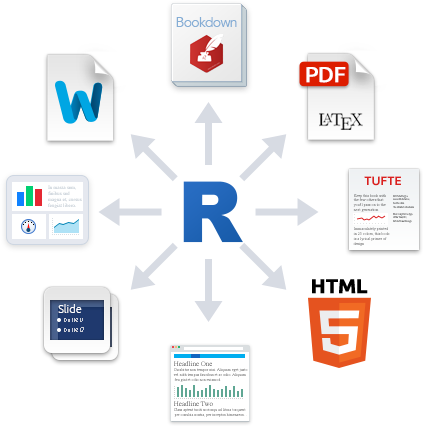
\includegraphics[width = 4.75cm]{Rlogotree.png}}
\institute{2018 US EPA \\ R User Group Workshop}
\date{11 Sept 2018}

\begin{document}
    \begin{frame}
        \maketitle
    \end{frame}

    \begin{frame}
        \frametitle{Table of Contents}
        \tableofcontents
    \end{frame}

\section{Agenda}

\begin{frame}{Time Frame \& Objectives}
\begin{exampleblock}{Using LaTeX and Markdown for Reproducible Research}
\begin{center}
    \begin{tabular}{c c c}
    Day & Time & Room \\
    \textbf{Tues, Sept 11} & \textbf{8:30-11:30am} & \textbf{C111C}
\end{tabular}
\end{center}
\end{exampleblock}

\begin{itemize}
    \item This 1/2-day workshop will provide attendees with hands-on experience
using the basics of LaTeX, Markdown, and the R package knitr.
    \item After attending this workshop, you will be able to use these tools to
facilitate reproducible reports and research with R.
\end{itemize}
% This would be a really good place to check that everyone has R and RStudio installed.
\end{frame}

\begin{frame}{Steps/Agenda}
We will try to use our three hours as effectively as possible.

\begin{exampleblock}{Rough Agenda}
\begin{tabular}{r|l}
    8:30 & System checks \\
    8:45 & LaTeX \\
    9:00 & Markdown \\
    9:15 & Using Markdown and LaTeX together \\
    9:30 & Reproducible Research \\
    9:45 & \emph{BREAK} \\
    10:00 & Dynamic documents with sweave and knitr \\
    10:30 & How Markdown and LaTeX can work with R
    \end{tabular}
\end{exampleblock}
\end{frame}

\section{LaTeX}
\begin{frame}{LaTeX}
    \begin{quote}
        TeX is usually pronounced tech, making \emph{lah}-teck, lah-\emph{teck}, and \emph{lay}-teck the logical choices; but language is not always logical, so \emph{lay}-\emph{tecks} is also possible.
    \end{quote}
    --- Leslie B. Lamport, original developer of \LaTeX{}
\end{frame}

\begin{frame}{LaTeX}
LaTeX is a tool for typesetting based on the idea that it is better to leave document design to document designers, and to let authors get on with writing documents. It is widely used in academia for the publication of scientific documents in many fields, including mathematics, statistics, computer science, engineering, chemistry, physics, economics, and political science.

\begin{enumerate}
    \item \textbf{TeX engines have excellent quality output.} This especially holds for complex documents such as those with mathematics, with many tables, or many cross-references or hyperlinks, or just with many pages.
    \item \textbf{TeX is fast.}
    \item \textbf{TeX is stable.} It will never eat your document. \emph{Ever.}
\end{enumerate}
--- \url{https://www.ctan.org/tex/}
\end{frame}

\begin{frame}[fragile]{LaTeX: Minimal example}
Here is a minimal example of a full document written in LaTeX.
\begin{exampleblock}{}
\begin{lstlisting}
\documentclass{article}
\title{A Minimal LaTeX Example}
\author{Emily Li}

\begin{document}
\maketitle

Hello world!

\end{document}
\end{lstlisting}
\end{exampleblock}
\end{frame}

\begin{frame}{Levels of LaTeX: A disambiguation}
\begin{alertblock}{There are too many words with ``TeX'' in them}
If you are wondering, \alert{\emph{``Should I use LaTeX or MiKTeX?''}}, allow us to clear that up. These two slides will cover four types of TeX-related terms: distributions, editors, engines, and formats.
\end{alertblock}
\begin{enumerate}
    \item \textbf{Distributions:} \textit{MiKTeX, TeX Live, etc.} This is TeX-related software to be downloaded and installed. When someone says, ``I need to install TeX on my machine,'' they're usually looking for a distribution.
    \item \textbf{Editors:} \textit{Emacs, TeXworks, TeXShop, TeXStudio, etc.} These editors are what you use to create a document file. Some (e.g., TeXShop) are devoted specifically to TeX, while others (e.g., Emacs) can be used to edit any sort of file.
\end{enumerate}
--- \url{http://www.tug.org/levels.html}
\end{frame}
\begin{frame}{Levels of LaTeX: A disambiguation}
\begin{enumerate}
\setcounter{enumi}{2}
    \item \textbf{Engines:} \textit{TeX, pdfTeX, XeTeX, LuaTeX, etc.} These are the executable binaries which implement different TeX variants. When someone says, ``TeX can't find my fonts,'' they usually mean an engine.
    \item \textbf{Formats:} \textit{LaTeX, plain TeX, etc.} These are the TeX-based languages in which one actually writes documents. When someone says, ``TeX is giving me a mysterious error,'' they usually mean a format. (Incidentally, ``LaTeX'' has meant ``LaTeX2e'' for many years now.)
\end{enumerate}
--- \url{http://www.tug.org/levels.html}
\end{frame}

\begin{frame}{LaTeX Distributions}
To compile LaTeX, your computer needs one of these TeX distributions installed:
\vspace{0.5cm}

\begin{center}
    \begin{tabular}{c l}
    \hline
    Distribution & Operating System \\
    \hline
    MiKTeX & Windows OS \\
    TeX Live & Linux and other UNIX-like systems \\
    MacTeX & Mac OS X
\end{tabular}
\end{center}

\vspace{0.25cm}
You can also use an on-line, ready-to-use option like \href{https://www.sharelatex.com/}{ShareLaTeX} or \href{https://www.overleaf.com/}{Overleaf}.
\end{frame}

\begin{frame}[fragile]{LaTeX: Revisiting the minimal example}
\begin{exampleblock}{Try compiling this LaTeX}
\begin{lstlisting}
\documentclass{article}
\title{A Minimal LaTeX Example}
\author{Emily Li}

\begin{document}
\maketitle

Hello world!

\end{document}
\end{lstlisting}
\end{exampleblock}
\end{frame}

\section{Markdown}

\section{Markdown \& LaTeX}

\section{Reproducible Research}
\begin{frame}{Reproducible Research}
        \begin{quote}
        An article about computational science in a scientific publication is not the scholarship itself, it is merely the advertising of the scholarship. The actual scholarship is the complete software development environment and the \textbf{complete set of instructions which generated the figures}.
    \end{quote}
    --- 1995, David L. Donoho, professor of statistics at Stanford University
    %Though Donoho was referring to computational science, journals in other data-driven fields such as biostatistics have been moving in the direction of reproducible research as well. Results from scientific research have to be reproducible to be trustworthy.
\end{frame}

\begin{frame}[fragile]{Reproducible Research}
This chunk of R code produces a figure that illustrates a simulation of Brownian motion for 100 steps.
        \begin{exampleblock}{Try running this in RStudio}
\begin{lstlisting}
set.seed(1213) # for reproducibility
x <- cumsum(rnorm(100))
plot(x, type = ''l'',
    ylab = ''$x_{i+1}=x_i+\\epsilon_{i+1}$'',
    xlab = ''step'')
\end{lstlisting}
        \end{exampleblock}
\end{frame}

\begin{frame}[fragile]{Reproducible Research}
        \begin{exampleblock}{}
\begin{lstlisting}
set.seed(1213) # for reproducibility
x <- cumsum(rnorm(100))
plot(x, type = ''l'',
    ylab = ''$x_{i+1}=x_i+\\epsilon_{i+1}$'',
    xlab = ''step'')
\end{lstlisting}
        \end{exampleblock}
To put this in a document by hand, we would have to open RStudio, paste the code into the R console to draw the plot, save it as a PDF or image file, then insert it into a document with \verb|\includegraphics{}| in LaTeX or 'Insert Image' in Word. This is both tedious and difficult for the author to maintain. If we want to change the figure, we have to update both the source code and the typesetting file.
\end{frame}

%    \begin{frame}[plain]{Plain frame}
%        This is a frame with plain style and it is numbered.
%    \end{frame}

%    \begin{frame}[t]
%        This frame has an empty title and is aligned to top.
%    \end{frame}

%    \begin{frame}[noframenumbering]{No frame numbering}
%        This frame is not numbered and is citing reference \cite{knuth74}.
%    \end{frame}

    \begin{frame}{Typesetting and Math}
        The packages \texttt{inputenc} and \texttt{FiraSans}\footnote{\url{https://fonts.google.com/specimen/Fira+Sans}}\textsuperscript{,}\footnote{\url{http://mozilla.github.io/Fira/}} are used to properly set the main fonts.
        \vfill
        This theme provides styling commands to typeset \emph{emphasized}, \alert{alerted}, \textbf{bold}, \textcolor{example}{example text}, \dots
        \vfill
        \texttt{FiraSans} also provides support for mathematical symbols:
        \begin{equation*}
            e^{i\pi} + 1 = 0.
        \end{equation*}
    \end{frame}

    \section{Section 2}
    \begin{frame}{Blocks}
        \begin{block}{Block}
            Text.
        \end{block}
        \pause
        \begin{alertblock}{Alert block}
            Alert \alert{text}.
        \end{alertblock}
        \pause
        \begin{exampleblock}{Example block}
            Example \textcolor{example}{text}.
        \end{exampleblock}
    \end{frame}

    \begin{frame}{Lists}
        \begin{columns}[t, onlytextwidth]
            \column{0.33\textwidth}
                Items:
                \begin{itemize}
                    \item Item 1
                    \begin{itemize}
                        \item Subitem 1.1
                        \item Subitem 1.2
                    \end{itemize}
                    \item Item 2
                    \item Item 3
                \end{itemize}

            \column{0.33\textwidth}
                Enumerations:
                \begin{enumerate}
                    \item First
                    \item Second
                    \begin{enumerate}
                        \item Sub-first
                        \item Sub-second
                    \end{enumerate}
                    \item Third
                \end{enumerate}

            \column{0.33\textwidth}
                Descriptions:
                \begin{description}
                    \item[First] Yes.
                    \item[Second] No.
                \end{description}
        \end{columns}
    \end{frame}

    \begin{frame}[focus]
        Thanks for using \textbf{Focus}!
    \end{frame}

%    \appendix
%    \begin{frame}{References}
%        \nocite{*}
%        \bibliography{demo_bibliography}
%        \bibliographystyle{plain}
%    \end{frame}

    \begin{frame}{Backup frame}
        \usebeamercolor[fg]{normal text}
        This is a backup frame, useful to include additional material for questions from the audience.
        \vfill
        The package \texttt{appendixnumberbeamer} is used not to number appendix frames.
    \end{frame}
\end{document}
